\documentclass[preview]{standalone}

\usepackage{amsmath}
\usepackage{amssymb}
\usepackage{stellar}
\usepackage{definitions}
\usepackage{bettelini}
\usepackage{tikz}

\begin{document}

\id{graph-spanning-trees-cayley-graphs}
\genpage

\section{Spanning trees}

\begin{snippetdefinition}{spanning-tree-definition}{Spanning tree}
    Let \(G\) be a connected \graph. A \emph{spanning tree} of \(G\) is a
    subgraph \(T\subseteq G\) such that \(T\) is a tree and
    \[
        V(T)=V(G).
    \]
    Thus \(T\) contains every vertex of \(G\), but not necessarily every edge.
\end{snippetdefinition}

\begin{snippetexample}{spanning-tree-example}{Spanning trees}
    A connected graph may have more than one spanning tree:
    \[
    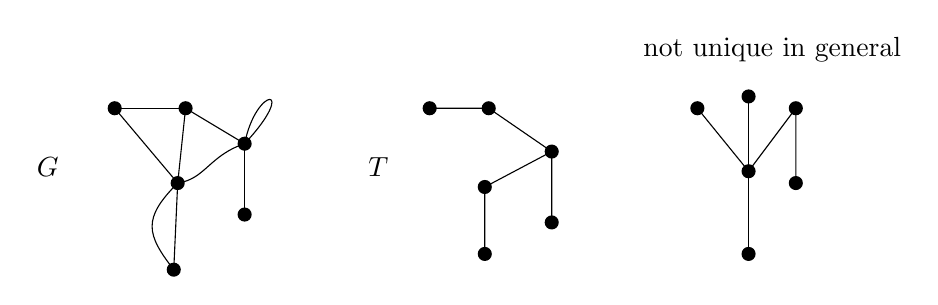
\begin{tikzpicture}[
        scale=1,
        line cap=round,
        line join=round,
        v/.style={circle, fill, inner sep=1.8pt}
    ]
        \begin{scope}
            \node at (-0.85,0.25) {\(G\)};

            \coordinate (g1) at (0,1);
            \coordinate (g2) at (0.9,1);
            \coordinate (g3) at (0.8,0.05);
            \coordinate (g4) at (1.65,0.55);
            \coordinate (g5) at (1.65,-0.35);
            \coordinate (g6) at (0.75,-1.05);

            \draw (g1)--(g2);
            \draw (g1)--(g3);
            \draw (g2)--(g3);
            \draw (g2)--(g4);
            \draw (g3) .. controls +(0.35,0.05) and +(-0.45,-0.15) .. (g4);
            \draw (g4)--(g5);
            \draw (g3)--(g6);
            \draw (g3) .. controls +(-0.45,-0.45) and +(-0.35,0.45) .. (g6);
            \draw (g4) .. controls +(0.15,0.75) and +(0.70,0.75) .. (g4);

            \foreach \p in {g1,g2,g3,g4,g5,g6}{
                \node[v] at (\p) {};
            }
        \end{scope}

        \begin{scope}[xshift=4cm]
            \node at (-0.65,0.25) {\(T\)};

            \coordinate (t1) at (0,1);
            \coordinate (t2) at (0.75,1);
            \coordinate (t3) at (0.70,0);
            \coordinate (t4) at (1.55,0.45);
            \coordinate (t5) at (1.55,-0.45);
            \coordinate (t6) at (0.70,-0.85);

            \draw (t1)--(t2)--(t4)--(t5);
            \draw (t4)--(t3)--(t6);

            \foreach \p in {t1,t2,t3,t4,t5,t6}{
                \node[v] at (\p) {};
            }
        \end{scope}

        \begin{scope}[xshift=7.4cm]
            \node at (0.95,1.75) {not unique in general};

            \coordinate (u0) at (0.65,0.2);
            \coordinate (u1) at (0,1);
            \coordinate (u2) at (0.65,1.15);
            \coordinate (u3) at (1.25,1);
            \coordinate (u4) at (1.25,0.05);
            \coordinate (u5) at (0.65,-0.85);

            \draw (u1)--(u0);
            \draw (u2)--(u0);
            \draw (u0)--(u3)--(u4);
            \draw (u0)--(u5);

            \foreach \p in {u0,u1,u2,u3,u4,u5}{
                \node[v] at (\p) {};
            }
        \end{scope}
    \end{tikzpicture}
    \]
\end{snippetexample}

\begin{snippetdefinition}{maximal-subtree-definition}{Maximal subtree}
    Let \(G\) be a \graph. A subtree \(T\) of \(G\) is \emph{maximal} if
    there is no subtree \(T'\) of \(G\) such that
    \[
        T\subsetneq T'.
    \]
    Maximality is with respect to inclusion of subgraphs, so both vertices and
    edges are compared.
\end{snippetdefinition}

\begin{snippetproposition}{spanning-tree-maximal-subtree-equivalence}{Spanning trees and maximal subtrees}
    Let \(G\) be a connected \graph and let \(T\) be a subtree of \(G\).
    Then \(T\) is a spanning tree of \(G\) \ifandonlyif \(T\) is maximal among
    the subtrees of \(G\).
\end{snippetproposition}

\begin{snippetproof}{spanning-tree-maximal-subtree-equivalence-proof}{spanning-tree-maximal-subtree-equivalence}{Spanning trees and maximal subtrees}
    \begin{iffproof}
        \item Suppose that \(T\) is a spanning tree of \(G\). Then
        \(V(T)=V(G)\). If \(T\) were not maximal, there would be a subtree
        \(T'\) of \(G\) such that \(T\subsetneq T'\). Since \(T\) already
        contains every vertex of \(G\), the subgraph \(T'\) must add at least
        one edge \(uv\notin E(T)\). The endpoints \(u\) and \(v\) lie in
        \(V(T)\). Since \(T\) is a tree, there is a path in \(T\) joining
        \(u\) and \(v\). Adding the edge \(uv\) creates a cycle, so \(T'\) is
        not a tree, contradiction. Hence \(T\) is maximal.

        \item Suppose that \(T\) is maximal among subtrees of \(G\). We show
        that \(V(T)=V(G)\). If some vertex \(v\in V(G)\setminus V(T)\)
        existed, choose a vertex \(u\in V(T)\). Since \(G\) is connected,
        there is a path in \(G\)
        \[
            u=x_0,x_1,\ldots,x_m=v.
        \]
        Let \(i\) be the first index such that \(x_i\notin V(T)\). Then
        \(x_{i-1}\in V(T)\) and the edge \(x_{i-1}x_i\) belongs to \(G\).

        Add the new vertex \(x_i\) and the edge \(x_{i-1}x_i\) to \(T\).
        This creates a strictly larger subtree of \(G\), because the new
        vertex is attached as a leaf. This contradicts maximality. Therefore
        \(V(T)=V(G)\), so \(T\) is spanning.
    \end{iffproof}
\end{snippetproof}

\begin{snippettheorem}{zorns-lemma}{Zorn's lemma}
    Let \(P\) be a non-empty partially ordered set. If every totally ordered
    subset \(S\subseteq P\) has an upper bound in \(P\), then \(P\) contains a
    maximal element.
\end{snippettheorem}

\begin{snippettheorem}{spanning-tree-existence-theorem}{Existence of spanning trees}
    Every non-empty connected \graph \(G\) admits a spanning tree.
\end{snippettheorem}

\begin{snippetproof}{spanning-tree-existence-proof}{spanning-tree-existence-theorem}{Existence of spanning trees}
    Let
    \[
        P=\{T\mid T \text{ is a subtree of } G\},
    \]
    ordered by inclusion. The set \(P\) is non-empty because any single vertex
    of \(G\), with no edges, is a tree.

    Let \(\mathcal{S}\subseteq P\) be a totally ordered subset, that is, a
    chain of subtrees of \(G\). Define \(T\) as the union of all subtrees in
    \(\mathcal{S}\):
    \[
        V(T)=\bigcup_{A\in\mathcal{S}} V(A),
        \qquad
        E(T)=\bigcup_{A\in\mathcal{S}} E(A).
    \]
    Then \(T\) is a subgraph of \(G\) containing every element of
    \(\mathcal{S}\). We show that \(T\) is a tree.

    First, \(T\) is connected. If \(u,v\in V(T)\), then there exist
    \(T_1,T_2\in\mathcal{S}\) such that \(u\in V(T_1)\) and \(v\in V(T_2)\).
    Since \(\mathcal{S}\) is totally ordered, either \(T_1\subseteq T_2\) or
    \(T_2\subseteq T_1\). In either case, \(u\) and \(v\) lie in one common
    subtree of the chain, and hence are connected in \(T\).

    Second, \(T\) has no cycles. If \(T\) contained a cycle \(C\), then \(C\)
    would use only finitely many edges \(e_1,\ldots,e_r\). For each \(e_i\),
    choose \(T_i\in\mathcal{S}\) containing \(e_i\). Since \(\mathcal{S}\) is
    a chain, one of the finitely many subtrees \(T_1,\ldots,T_r\) contains all
    the others. That subtree would contain the whole cycle \(C\), impossible
    because it is a tree.

    Therefore \(T\) is a tree, so it is an upper bound for \(\mathcal{S}\) in
    \(P\). By Zorn's lemma, \(P\) has a maximal element. By the equivalence
    between spanning trees and maximal subtrees, this maximal subtree is a
    spanning tree of \(G\).
\end{snippetproof}

\section{Cayley graphs}

\begin{snippetdefinition}{cayley-graph-definition}{Cayley graph}
    Let \(G\) be a \group and let \(S\subseteq G\).
    The \emph{Cayley graph} of \(G\) with respect to \(S\), denoted
    \[
        \operatorname{Cay}(G,S),
    \]
    is the \graph defined as follows:
    \begin{itemize}
        \item the vertices are the elements of \(G\);
        \item the edges are the elements of \(G\cartesianprod S\);
        \item the edge \((g,s)\in G\cartesianprod S\) has endpoints \(g\)
        and \(gs\).
    \end{itemize}
    This definition gives an undirected graph, possibly with loops and multiple
    edges.
\end{snippetdefinition}

\begin{snippetexample}{cayley-graph-cyclic-group-example}{Cayley graph of a cyclic group}
    Let \(G=\langle g\rangle\) be a cyclic group generated by \(g\), and let
    \(S=\{g\}\).

    If \(G\) is finite of order \(n\geq 3\), then the vertices are
    \[
        1,g,g^2,\ldots,g^{n-1},
    \]
    and the edge \((g^k,g)\) joins \(g^k\) to \(g^{k+1}\), with exponents read
    modulo \(n\). Thus the Cayley graph is a cycle.

    \[
        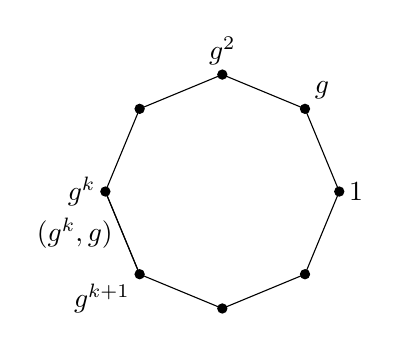
\begin{tikzpicture}[scale=1.1]
            \foreach \i in {0,...,7}{
                \coordinate (v\i) at ({360/8*\i}:1.35);
                \fill (v\i) circle (1.7pt);
            }

            \foreach \i/\j in {0/1,1/2,2/3,3/4,4/5,5/6,6/7,7/0}{
                \draw (v\i)--(v\j);
            }

            \node[right] at (v0) {\(1\)};
            \node[above right] at (v1) {\(g\)};
            \node[above] at (v2) {\(g^2\)};
            \node[left] at (v4) {\(g^k\)};
            \node[below left] at (v5) {\(g^{k+1}\)};

            \draw (v4)--node[left] {\((g^k,g)\)} (v5);
        \end{tikzpicture}
    \]

    If \(G\) is infinite, the Cayley graph is a bi-infinite line:
    \[
        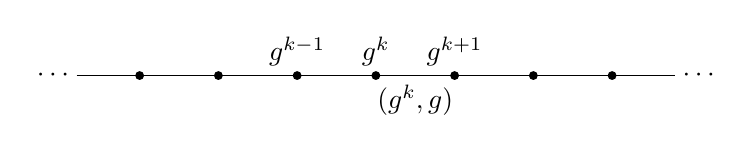
\begin{tikzpicture}[scale=1]
            \foreach \x in {-3,-2,-1,0,1,2,3}{
                \fill (\x,0) circle (1.6pt);
            }

            \draw (-3.8,0)--(3.8,0);
            \node at (-4.1,0) {\(\cdots\)};
            \node at (4.1,0) {\(\cdots\)};

            \node[above] at (-1,0) {\(g^{k-1}\)};
            \node[above] at (0,0) {\(g^k\)};
            \node[above] at (1,0) {\(g^{k+1}\)};

            \node[below] at (0.5,0) {\((g^k,g)\)};
        \end{tikzpicture}
    \]
\end{snippetexample}

\begin{snippetproposition}{cayley-graph-loops-multiple-edges}{Loops and multiple edges in Cayley graphs}
    Let \(\operatorname{Cay}(G,S)\) be a Cayley graph.
    Then:
    \begin{itemize}
        \item loops occur \ifandonlyif \(1_G\in S\);
        \item multiple edges occur \ifandonlyif there exists \(s\in S\) such
        that \(s^{-1}\in S\). This includes the case \(s=s^{-1}\), that is,
        \(s^2=1_G\).
    \end{itemize}
\end{snippetproposition}

\begin{snippetproof}{cayley-graph-loops-multiple-edges-proof}{cayley-graph-loops-multiple-edges}{Loops and multiple edges in Cayley graphs}
    The edge \((g,s)\) is a loop \ifandonlyif its endpoints coincide:
    \[
        g=gs.
    \]
    Multiplying on the left by \(g^{-1}\), this is equivalent to \(s=1_G\).
    Hence loops occur precisely when \(1_G\in S\).

    For multiple edges, suppose \(s,s^{-1}\in S\). The edge \((g,s)\) joins
    \(g\) to \(gs\), while the edge \((gs,s^{-1})\) joins \(gs\) to
    \[
        (gs)s^{-1}=g.
    \]
    These are distinct edges with the same endpoints.

    Conversely, if two distinct edges have the same endpoints, then one of
    them corresponds to multiplication by some \(s\in S\), and the other to
    the inverse multiplication by \(s^{-1}\). Hence \(s^{-1}\in S\).
\end{snippetproof}

\begin{snippetexample}{cayley-graph-loops-multiple-edges-example}{Loops and multiple edges}
    If \(1_G\in S\), then each vertex \(g\) has the loop \((g,1_G)\):
    \[
        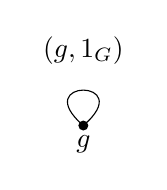
\begin{tikzpicture}[scale=1]
            \coordinate (g) at (0,0);
            \fill (g) circle (1.8pt);
            \node[below] at (g) {\(g\)};
            \draw (g) .. controls +(-0.7,0.6) and +(0.7,0.6) .. (g);
            \node[above] at (0,0.65) {\((g,1_G)\)};
        \end{tikzpicture}
    \]
    If \(s,s^{-1}\in S\), then two distinct edges have the same endpoints:
    \[
        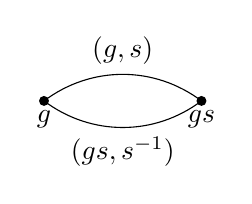
\begin{tikzpicture}[scale=1]
            \coordinate (g) at (0,0);
            \coordinate (h) at (2,0);

            \fill (g) circle (1.8pt);
            \fill (h) circle (1.8pt);

            \node[below] at (g) {\(g\)};
            \node[below] at (h) {\(gs\)};

            \draw (g) .. controls +(0.6,0.45) and +(-0.6,0.45) .. node[above] {\((g,s)\)} (h);
            \draw (g) .. controls +(0.6,-0.45) and +(-0.6,-0.45) .. node[below] {\((gs,s^{-1})\)} (h);
        \end{tikzpicture}
    \]
\end{snippetexample}

\begin{snippetproposition}{cayley-graph-connected-components}{Connected components of a Cayley graph}
    Let \(G\) be a \group, let \(S\subseteq G\), and put
    \[
        H=\langle S\rangle.
    \]
    The connected component of a vertex \(g\in G\) in
    \(\operatorname{Cay}(G,S)\) has vertex set
    \[
        gH.
    \]
    In particular, the connected component of \(1_G\) has vertex set
    \(\langle S\rangle\). Hence
    \[
        \operatorname{Cay}(G,S) \text{ is connected}
        \quad\Longleftrightarrow\quad
        G=\langle S\rangle.
    \]
\end{snippetproposition}

\begin{snippetproof}{cayley-graph-connected-components-proof}{cayley-graph-connected-components}{Connected components of a Cayley graph}
    An edge of the Cayley graph allows one to pass from a vertex \(x\) to
    \(xs\), where \(s\in S\). Since the graph is undirected, traversing the
    same edge in the opposite direction corresponds to multiplying on the
    right by \(s^{-1}\).

    Therefore, a path from \(g\) to \(h\) corresponds to an expression
    \[
        h=g s_1s_2\cdots s_r,
    \]
    where each \(s_i\) lies in \(S\union S^{-1}\). Equivalently,
    \[
        g^{-1}h=s_1s_2\cdots s_r\in\langle S\rangle.
    \]
    Thus \(h\in g\langle S\rangle\).

    Conversely, if \(h\in g\langle S\rangle\), then
    \[
        h=g s_1s_2\cdots s_r
    \]
    for some \(s_i\in S\union S^{-1}\). Each right multiplication by \(s_i\)
    corresponds to traversing an edge, possibly in the reverse direction.
    Hence there is a path from \(g\) to \(h\).

    The connected component of \(g\) is therefore \(g\langle S\rangle\). The
    Cayley graph is connected \ifandonlyif every element of \(G\) belongs to
    the component of \(1_G\), which is equivalent to \(G=\langle S\rangle\).
\end{snippetproof}

\begin{snippetcorollary}{cayley-graph-components-as-cosets}{Components as cosets}
    Let \(G\) be a \group and let \(S\subseteq G\).
    The connected components of \(\operatorname{Cay}(G,S)\) are the left
    cosets of \(\langle S\rangle\):
    \[
        g\langle S\rangle,
        \qquad g\in G.
    \]
\end{snippetcorollary}

\begin{snippetproposition}{cayley-graph-circuits}{Circuits in Cayley graphs}
    Let \(G\) be a \group and let \(S\subseteq G\).
    The Cayley graph \(\operatorname{Cay}(G,S)\) contains a circuit
    \ifandonlyif there exists a non-trivial word
    \[
        s_1s_2\cdots s_r=1_G,
        \qquad
        s_i\in S\union S^{-1},
    \]
    with no immediate cancellations, meaning
    \[
        s_i s_{i+1}\neq 1_G
        \quad
        \text{for every } i.
    \]
    To obtain a simple circuit, one also requires the partial products
    \[
        1_G,\ s_1,\ s_1s_2,\ \ldots,\ s_1s_2\cdots s_{r-1}
    \]
    to be distinct.
\end{snippetproposition}

\begin{snippetproof}{cayley-graph-circuits-proof}{cayley-graph-circuits}{Circuits in Cayley graphs}
    Suppose that
    \[
        s_1s_2\cdots s_r=1_G,
        \qquad
        s_i\in S\union S^{-1}.
    \]
    Starting from a vertex \(g\), consider the sequence of vertices
    \[
        g,\quad
        gs_1,\quad
        gs_1s_2,\quad
        \ldots,\quad
        gs_1s_2\cdots s_r.
    \]
    Since \(s_1s_2\cdots s_r=1_G\), the final vertex is again \(g\), so this
    gives a closed walk.

    The condition \(s_i s_{i+1}\neq 1_G\) prevents the walk from traversing an
    edge and immediately traversing the same edge back. If the partial products
    are distinct, no intermediate vertex is repeated, so the closed walk is a
    simple circuit.

    Conversely, every circuit in the Cayley graph determines a sequence of
    right multiplications by elements of \(S\union S^{-1}\). Since the circuit
    returns to its starting vertex, the corresponding product is \(1_G\).
\end{snippetproof}

\end{document}
